\chapter{Drake Simulation}

\section{Overview and objectives}

Instead of building a set of equations to simulate a robot from scratch, designers can use existing tools to simplify and streamline the modelling of a robot's movement. One such tool is rigid body simulation, which involves placing objects in a simulated environment and modelling the weights, joints, and contact forces of each object. This project uses rigid body simulation to model the motion of the device, with the objective to inform designers on how the device will move. By using established simulation software, it is easier to model the device using fewer assumptions than in the maths model, leading to a more accurate system.\\
\\
\section{Selection of simulator}
The simulation programs considered in this project are PyBullet, Gazebo, and Drake. Each of these have their own advantages but Drake was selected due to its focus on accurate multibody and friction simulation.
\\
Drake is a multibody physics engine developed and used by MIT. This project uses Drake's python bindings which are available in the package "pydrake", which runs on Ubuntu using Windows Subsystem for Linux (WSL).\\
\section{CAD to simulation pipeline}
To model a robot, Drake requires a simulation description format file (SDFormat). Currently, not many CAD programs provide a method to easily generate these files. This project used Onshape, a cloud-based CAD program, for this reason. The python library, onshape-to-robot, is then used to build an SDFormat file. The generated SDFormat file is then modified in order to meet Drake's specific requirements, and to apply realistic coefficients of friction to the wheels and tail.\\

\section{Using the simulator}
Once the robot has been loaded into the multibody simulation, it can be driven by setting a torque on the motor joints. Simply setting the torque on the joint to a constant value would cause the device to accelerate continuously ad infinitum. DC motor torque decreases as the speed increases until the torque reaches an equilibrium with the resistive forces and a constant speed is achieved. The following equation models the toque output of a geared DC motor.\\

$Torque = StallTorque*(Voltage/12.0-speed/NLSpeed)$\\

This essentially acts as a high-gain proportional speed controller. The motor voltage is set through sliders in the simulator options. \\
The device can now be tested in simulation to determine whether it can climb stairs, and to gain insight into which components make contact with the stairs and when. Figure \ref{fig:simulation-screenshot} shows the device climbing a set of stairs in the Drake simulator.\\

\begin{figure}[h]
	\centering
	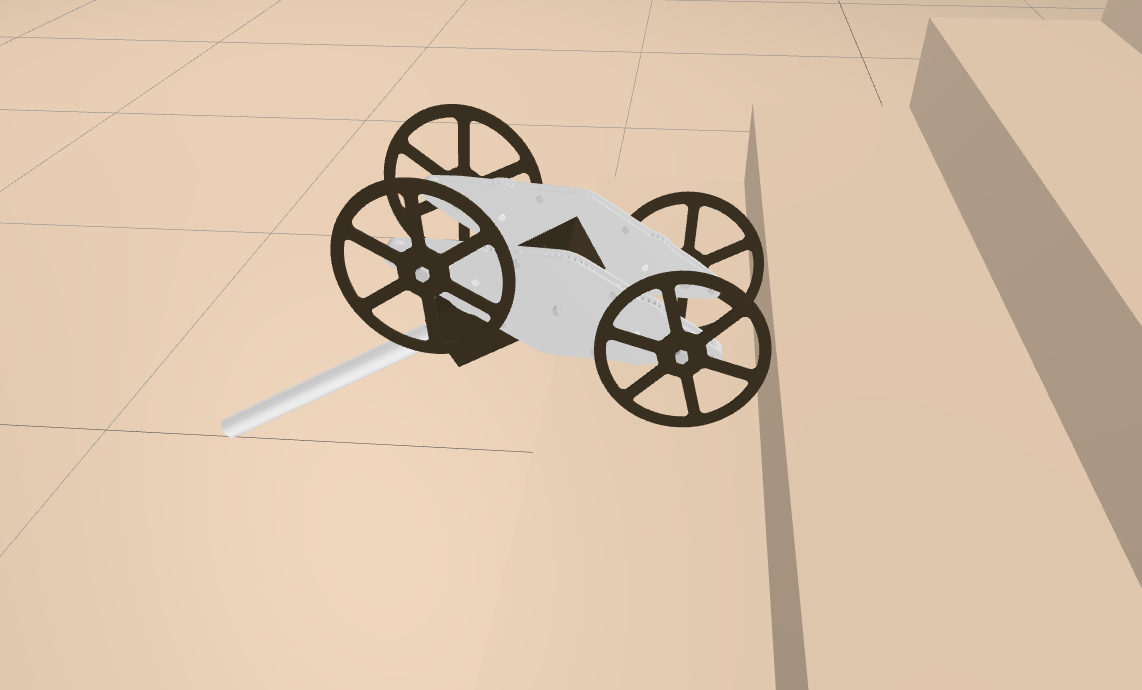
\includegraphics[width=0.8\textwidth]{simulation-screenshot}
	\caption{Screenshot of the device climbing steps in the Drake simulation.}
	\label{fig:simulation-screenshot}
\end{figure}